% =============================================================================================
%  COM 837 - Assignment 3 report.  Compile with pdflatex (Overleaf: upload report.tex + figures/).
%  Tables can be regenerated after a new run with   python scripts/s7_latex_tables.py
% =============================================================================================
\documentclass[10pt,a4paper]{article}

\usepackage[utf8]{inputenc}
\usepackage[T1]{fontenc}
\usepackage{lmodern}
\usepackage[margin=1.8cm]{geometry}
\usepackage{amsmath,amssymb}
\usepackage{graphicx}
\usepackage{booktabs}
\usepackage{multirow}
\usepackage{caption}
\usepackage{subcaption}
\usepackage[compact]{titlesec}
\usepackage{enumitem}
\usepackage{xcolor}
\usepackage{microtype}
\usepackage[colorlinks=true,linkcolor=blue!50!black,citecolor=blue!50!black,urlcolor=blue!50!black]{hyperref}
\urlstyle{same}

\captionsetup{font=small,labelfont=bf,skip=3pt}
\captionsetup[sub]{font=small,skip=1pt}
\setlist{itemsep=1pt,topsep=2pt,parsep=0pt,leftmargin=*}
\setlength{\textfloatsep}{8pt plus 2pt minus 2pt}
\setlength{\floatsep}{6pt plus 2pt minus 2pt}
\setlength{\intextsep}{6pt plus 2pt minus 2pt}
\setlength{\abovedisplayskip}{4pt}
\setlength{\belowdisplayskip}{4pt}
\setlength{\parskip}{2pt}
\renewcommand{\arraystretch}{1.05}

\newcommand{\studentname}{Jagini Mohit}
\newcommand{\rollno}{IMT2023528}
\newcommand{\HLS}{\mathbf{h}_{\mathrm{LS}}}
\newcommand{\code}[1]{\texttt{\small #1}}

\title{\vspace{-1.2cm}\textbf{ChannelNet: OFDM Channel Estimation by Image Super-Resolution\\and Image Restoration}}
\author{COM 837 -- Machine Learning for Wireless Communication -- Assignment 3\\
Name: \studentname \qquad Roll No.: \rollno\\
Code repository: \url{https://github.com/Mohit14036/MLWCAssignment}}
\date{\vspace{-0.9cm}}

\begin{document}
\maketitle

% ---------------------------------------------------------------------------------------------
\section{Objective}

One LTE sub-frame of a SISO-OFDM link spans $72$ sub-carriers and $14$ OFDM symbols. Its channel
response $H[k,l]$ can therefore be viewed as a $72\times14$ image, of which the receiver only sees a
few noisy pixels: the least-squares (LS) estimates at the pilot positions. Following Soltani
\emph{et al.}~\cite{soltani}, I rebuild the full image with \textbf{ChannelNet}, a super-resolution
network (SRCNN~\cite{srcnn}) followed by a denoising network (DnCNN~\cite{dncnn}). ChannelNet is compared
with LS + 2-D interpolation and with the three MMSE-type baselines of the paper (ideal MMSE, estimated
MMSE, ideal ALMMSE~\cite{simko}) on the Vehicular-A (VehA) and SUI5 channels, for SNRs of 0--30~dB and
8--48 pilots per sub-frame.

% ---------------------------------------------------------------------------------------------
\section{System model and data generation (Task 1)}

\paragraph{OFDM grid.} I use the LTE 1.4~MHz numerology: 72 active sub-carriers (DC left empty), 15~kHz
spacing, $N_{\mathrm{FFT}}=128$, normal cyclic prefix (CP) and 14 symbols per 1~ms sub-frame. If the
CP is longer than the channel and the channel does not change within one symbol, each resource element
obeys (eqs.~(1)--(2) of~\cite{soltani})
\begin{equation}
  Y[k,l] = H[k,l]\,X[k,l] + Z[k,l],\quad Z\sim\mathcal{CN}(0,\sigma^2),\quad
  \mathrm{SNR}=\frac{\mathbb{E}|X|^2\,\mathbb{E}|H|^2}{\sigma^2}=\frac{1}{\sigma^2},\qquad
  \hat H_{\mathrm{LS}}[k_p,l_p] = \frac{Y[k_p,l_p]}{X[k_p,l_p]}.
\end{equation}
\code{tests/test\_ofdm\_link.py} confirms this model with a complete time-domain link (IFFT, CP,
convolution with the impulse response, CP removal, FFT). The two agree to $10^{-15}$.

\paragraph{Channel models.} Both channels are WSSUS tapped-delay lines sampled at sub-carrier
frequency $f_k$ and symbol centre $t_l$:
$H[k,l]=\sum_p\sqrt{P_p}\,g_p(t_l)\,e^{-j2\pi f_k\tau_p}$, $\sum_p P_p=1$. Each tap has its own
unit-power Rayleigh process $g_p(t)$ with a Jakes spectrum, generated with the sum-of-sinusoids model
of Zheng and Xiao~\cite{zheng}. The carrier (2.1~GHz) and speed (50~km/h) follow the paper, giving
$f_D=97.3$~Hz and a coherence time of 4.3~ms. \textbf{VehA} (ITU-R M.1225) has 6 taps between 0 and
2.51~$\mu$s, an RMS delay spread of 0.37~$\mu$s and a coherence bandwidth of 540~kHz.
\textbf{SUI5} has taps at 0/4/10~$\mu$s with powers 0/$-5$/$-10$~dB, an RMS delay spread of 2.84~$\mu$s
and a coherence bandwidth of only 70~kHz, about 5 sub-carriers. Its 10~$\mu$s excess delay is also
longer than the 4.7~$\mu$s CP. SUI5 is therefore far more frequency-selective than VehA (Fig.~\ref{fig:gt}).

\paragraph{Simulator.} The paper used the Vienna LTE-A simulator; the course supplied the
\textbf{Vienna 5G Link-Level Simulator}. \code{matlab/make\_vienna\_dataset.m} uses its
\code{Channel.FastFading} class (15.36~MHz sampling, built-in VehicularA profile, SUI5 as a
user-defined profile). It reads \code{GetTransferFunction} at the centre of every OFDM symbol on the 72
active bins. For training on Kaggle I used the Python implementation of the same models
(\code{chnet/channels.py}). Its statistics agree with the Vienna channels: the correlation between
sub-carriers 6 apart is 0.979 (VehA) and 0.634 (SUI5) in theory, against 0.973 and 0.653 measured on
the Vienna frames. The correlation between the first and last symbol of the sub-frame is
$J_0(2\pi f_D\cdot0.93\,\mathrm{ms})=0.92$ for both. Section~\ref{sec:vienna} also tests the trained
networks directly on Vienna channels.

\paragraph{Pilots and data set.} All pilot patterns are lattices (Fig.~\ref{fig:pilots}). The main
pattern has \textbf{48 pilots}: OFDM symbols $\{0,4,7,11\}$, every 6th sub-carrier, with the start
shifted by 3 on alternate pilot symbols (the LTE CRS diamond). The other densities are 36 (spacing 8,
baselines only), 24 (symbols $\{3,10\}$, spacing 6), 16 (spacing 9) and 8 (spacing 18). All
pilots are unit-energy QPSK. Each channel has 40\,000 frames, split 32\,000/4\,000/4\,000 into
training, validation and test sets as in the paper. Every random quantity comes from its own stream,
derived from the master seed and a tag such as (noise, VehA, test, 48, 22~dB) (\code{chnet/rng.py}).
All estimators therefore see exactly the same noisy pilots. Each complex grid becomes \textbf{two
real images} (real and imaginary part), divided by the standard deviation of the training entries
(0.707).

\begin{figure}[!htbp]
  \centering
  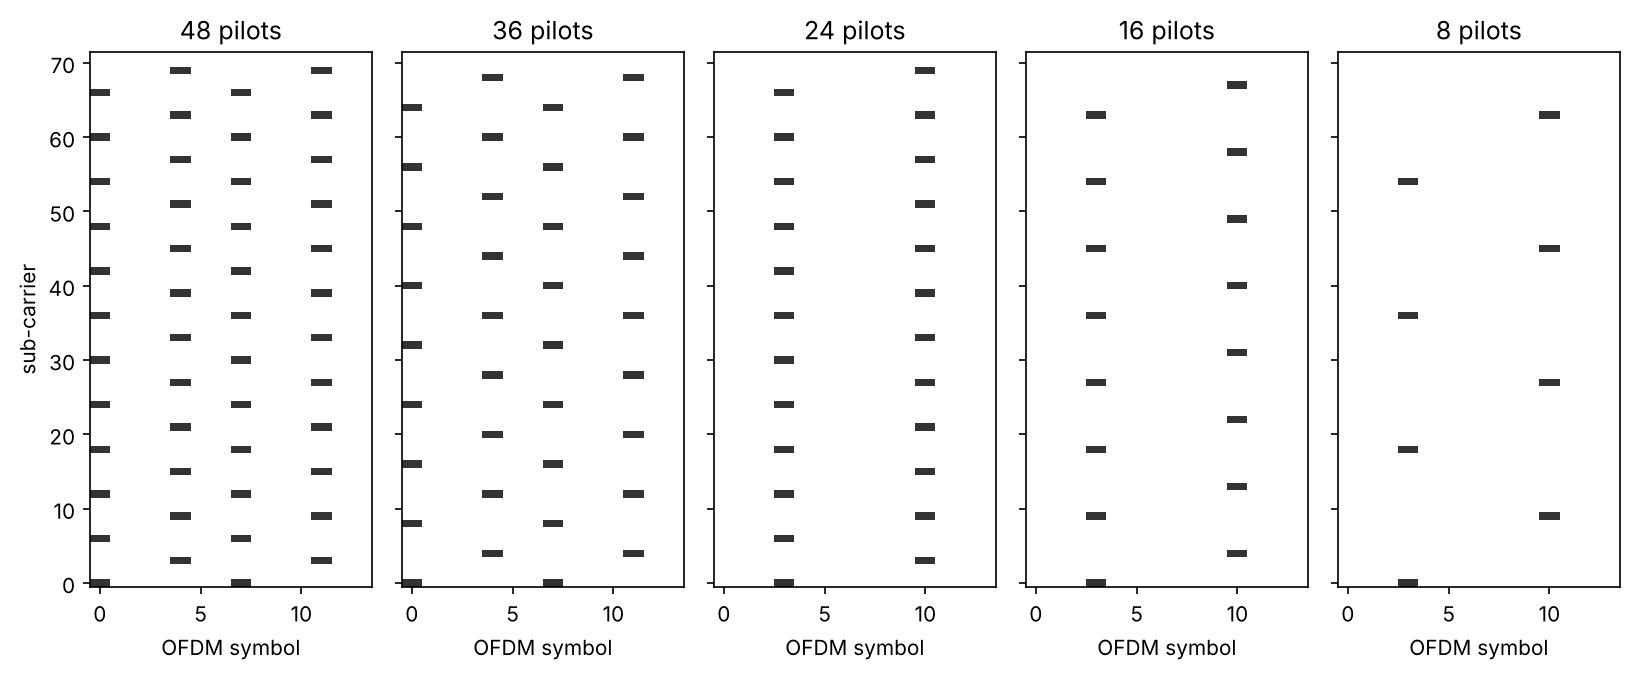
\includegraphics[width=0.66\textwidth]{figures/pilot_patterns.png}
  \caption{Lattice pilot patterns on the $72\times14$ grid (black = pilot).}
  \label{fig:pilots}
\end{figure}

\begin{figure}[!htbp]
  \centering
  \begin{subfigure}[t]{0.42\textwidth}
    \centering
    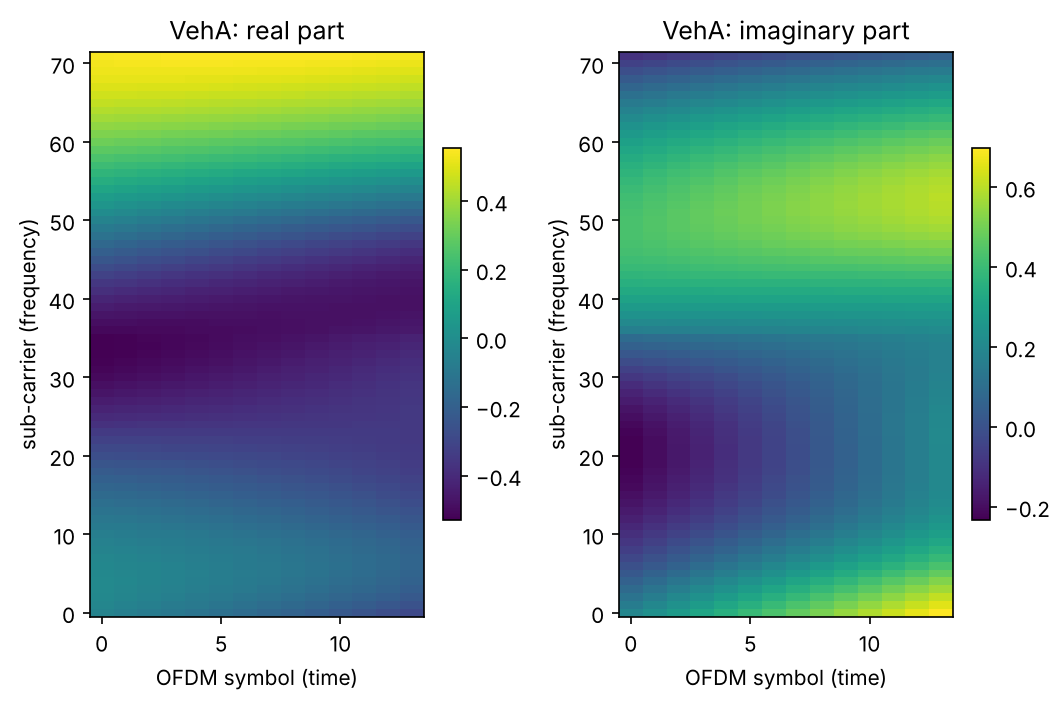
\includegraphics[width=\linewidth]{figures/fig2_ground_truth_VehA.png}
    \caption{VehA: smooth in both time and frequency.}
  \end{subfigure}\hspace{0.04\textwidth}
  \begin{subfigure}[t]{0.42\textwidth}
    \centering
    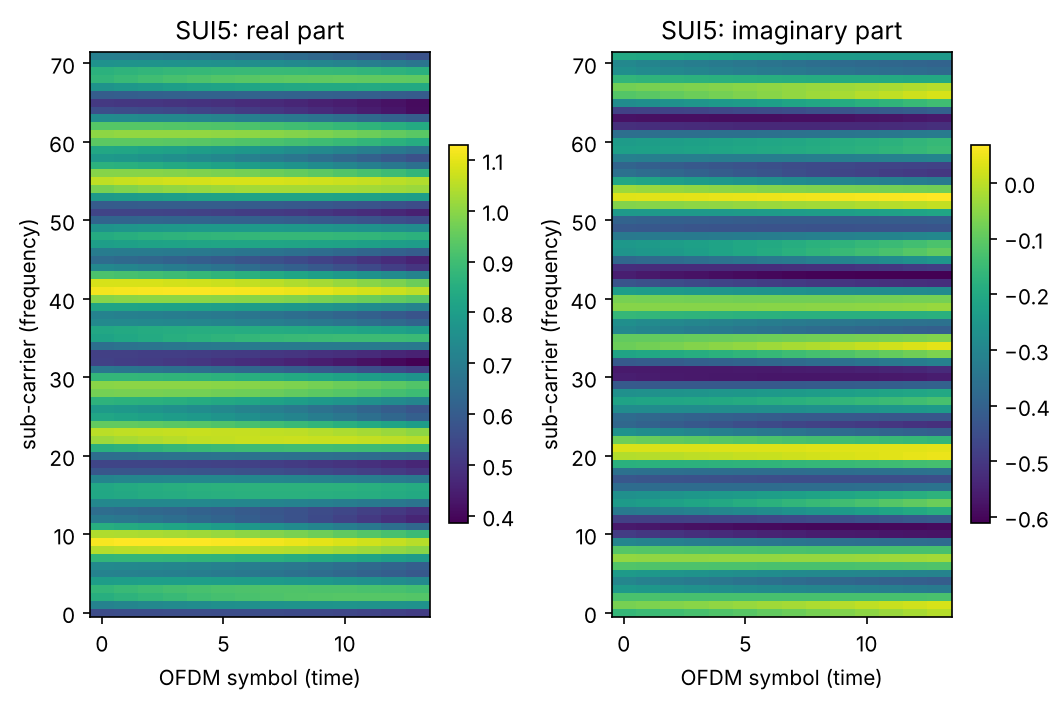
\includegraphics[width=\linewidth]{figures/fig2_ground_truth_SUI5.png}
    \caption{SUI5: rapid ripples along frequency.}
  \end{subfigure}
  \caption{Real and imaginary parts of a ground-truth channel (cf.\ Fig.~1 of~\cite{soltani}).}
  \label{fig:gt}
\end{figure}

% ---------------------------------------------------------------------------------------------
\section{Conventional channel estimation (Task 2)}

The pilot positions are fixed, so every conventional estimator is linear in the LS pilot vector:
$\hat{\mathbf h}=\mathbf W\HLS$ with $\mathbf W\in\mathbb C^{1008\times P}$. \code{chnet/classical.py}
builds one matrix per method and SNR.
\begin{itemize}
  \item \textbf{LS + 2-D interpolation}: piecewise-linear (Delaunay), cubic (Clough--Tocher) and
    Gaussian radial-basis-function interpolation over the (sub-carrier, symbol) plane. The RBF variant
    is the one used in the reference code of the paper. Grid points outside the convex hull of the
    pilots take the value of the nearest pilot.
  \item \textbf{Ideal MMSE} (eq.~(5) of~\cite{soltani}): $\hat{\mathbf h}=\mathbf R_{hp}(\mathbf R_{pp}
    +\sigma^2\mathbf I)^{-1}\HLS$, using the exact $1008\times1008$ covariance of the 32\,000 true
    training channels. Because it needs the true statistics, it serves as the genie lower bound.
  \item \textbf{Estimated MMSE}: the same filter, but with a covariance learned from 2\,000
    \emph{received} frames at the operating SNR (LS pilots + linear interpolation). The known noise
    contribution $\sigma^2\mathbf W_{\mathrm{lin}}\mathbf W_{\mathrm{lin}}^T$ is subtracted.
  \item \textbf{Ideal ALMMSE} (\v{S}imko \emph{et al.}~\cite{simko}): assumes a separable correlation
    $\mathbf R_h=\mathbf R_{\mathrm{time}}\otimes\mathbf R_{\mathrm{freq}}$ and filters the interpolated LS
    grid in frequency and then in time, $\hat{\mathbf H}=\mathbf B_{\mathrm{freq}}\hat{\mathbf
    H}_{\mathrm{int}}\mathbf C_{\mathrm{time}}^T$. The filters come from a rank-one approximation of the
    per-eigenmode Wiener gains, keeping $N_{\mathrm{freq}}=5$ and $N_{\mathrm{time}}=2$ eigenvalues.
\end{itemize}

% ---------------------------------------------------------------------------------------------
\section{ChannelNet (Tasks 3 and 4)}

The LS pilot values are first interpolated onto the full grid with the Gaussian RBF, as in the paper.
This gives the low-resolution image. The SRCNN maps it to a full-resolution estimate, and the
cascaded DnCNN then removes the remaining noise by predicting it and subtracting it (residual
learning): $\hat{\mathbf H}=f_{\mathrm{IR}}(f_{\mathrm{SR}}(\mathrm{interp}(\hat{\mathbf H}_{\mathrm{LS}})))$.
The real and imaginary parts are processed as separate single-channel images. All convolutions use
zero `same' padding, so every feature map stays $72\times14$ (Table~\ref{tab:arch}). The SRCNN has
8\,129 parameters and the DnCNN 0.67\,M (\code{chnet/nets.py}). The last DnCNN layer starts at zero,
so the IR stage begins as the identity mapping.

\begin{table}[!htbp]
  \centering
  \caption{ChannelNet architecture (as in the paper).}
  \label{tab:arch}
  \small
  \begin{tabular}{llccl}
    \toprule
    stage & layer & kernel & filters & activation \\
    \midrule
    SR (SRCNN) & conv 1 / 2 / 3 & $9\times9$ / $1\times1$ / $5\times5$ & 64 / 32 / 1 & ReLU / ReLU / linear \\
    \midrule
    \multirow{3}{*}{IR (DnCNN, 20 layers)} & conv 1 & $3\times3$ & 64 & ReLU \\
     & conv 2--19 & $3\times3$ & 64 & BN + ReLU \\
     & conv 20 & $3\times3$ & 1 & residual: $\hat{\mathbf x} = \mathbf y - \mathcal R(\mathbf y)$ \\
    \bottomrule
  \end{tabular}
\end{table}

% ---------------------------------------------------------------------------------------------
\section{Training procedure and reproducibility (Task 5)}

\begin{itemize}
  \item \textbf{Two training stages} (eqs.~(7)--(8) of~\cite{soltani}, \code{scripts/s4\_train.py}).
    The SRCNN is trained first with
    $C_1=\frac{1}{|\mathcal T|}\sum_i\|f_{\mathrm{SR}}(\mathbf X_i^{\mathrm{LR}})-\mathbf H_i\|_F^2$.
    It is then frozen, and the DnCNN is trained on its outputs with
    $C_2=\frac{1}{|\mathcal T|}\sum_i\|f_{\mathrm{IR}}(f_{\mathrm{SR}}(\mathbf X_i^{\mathrm{LR}}))-\mathbf H_i\|_F^2$.
    As in the paper I use Adam with learning rate $10^{-3}$ and batch size 128. The learning rate is
    halved when the validation loss stops improving, and early stopping on the validation loss keeps
    the best weights. The epoch limits are 150 (SR) and 40 (IR).
  \item \textbf{SNR-specific training}, as in the paper. A ``deep low-SNR'' network is trained at
    \textbf{12~dB} and a ``deep high-SNR'' network at \textbf{22~dB}; both are tested over 0--30~dB.
    The pilot study uses 22~dB networks for 48/24/16/8 pilots. A further \emph{multi-SNR} network,
    trained with a fresh SNR $\sim\mathcal U[0,30]$~dB per frame, tests one remedy for the SNR problem
    (Section~\ref{sec:discussion}). 14 ChannelNets were trained in total.
  \item \textbf{Cost and convergence.} Training ran on a Kaggle Tesla T4 with PyTorch and fp16 mixed
    precision, taking 23--33~min per network and 424~min in total. The SR stage usually reached its
    150-epoch limit while still improving slowly; the DnCNN converged within 17--40 epochs.
    Training and validation losses stay close throughout (Fig.~\ref{fig:loss}), so there is no
    overfitting with 64\,000 training images, and the IR stage clearly lowers the loss further.
  \item \textbf{Reproducibility.} One master seed (2026) generates every random stream: channels,
    noise, weight initialisation and batch order. cuDNN runs in deterministic mode and all settings
    live in \code{configs/experiment.yaml}. Each trained network is saved as
    \code{models/<channel>\_P<pilots>\_snr<S>/\{sr.pt, ir.pt, info.json\}}; \code{info.json} records the
    configuration, seed, normalisation scale and software versions. Training (\code{s4\_train.py}) and
    testing (\code{s5\_test.py}) are separate scripts, and testing only loads saved checkpoints.
\end{itemize}

\begin{figure}[!htbp]
  \centering
  \begin{subfigure}[t]{0.49\textwidth}
    \centering
    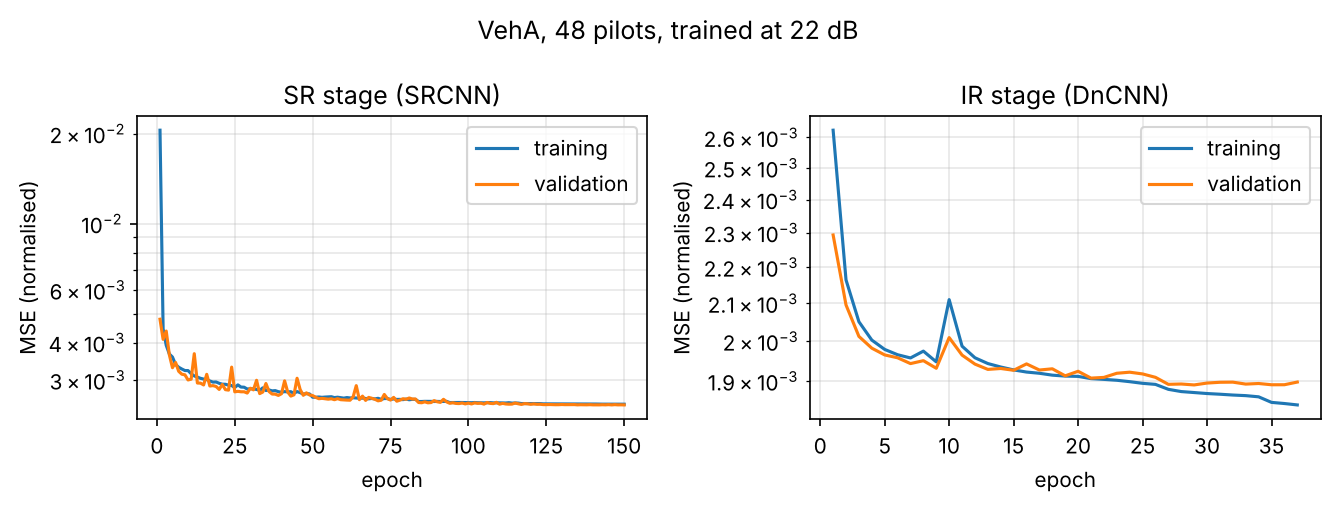
\includegraphics[width=\linewidth]{figures/loss_curves/loss_VehA_p48_snr22.png}
    \caption{VehA, 48 pilots, 22~dB.}
  \end{subfigure}\hfill
  \begin{subfigure}[t]{0.49\textwidth}
    \centering
    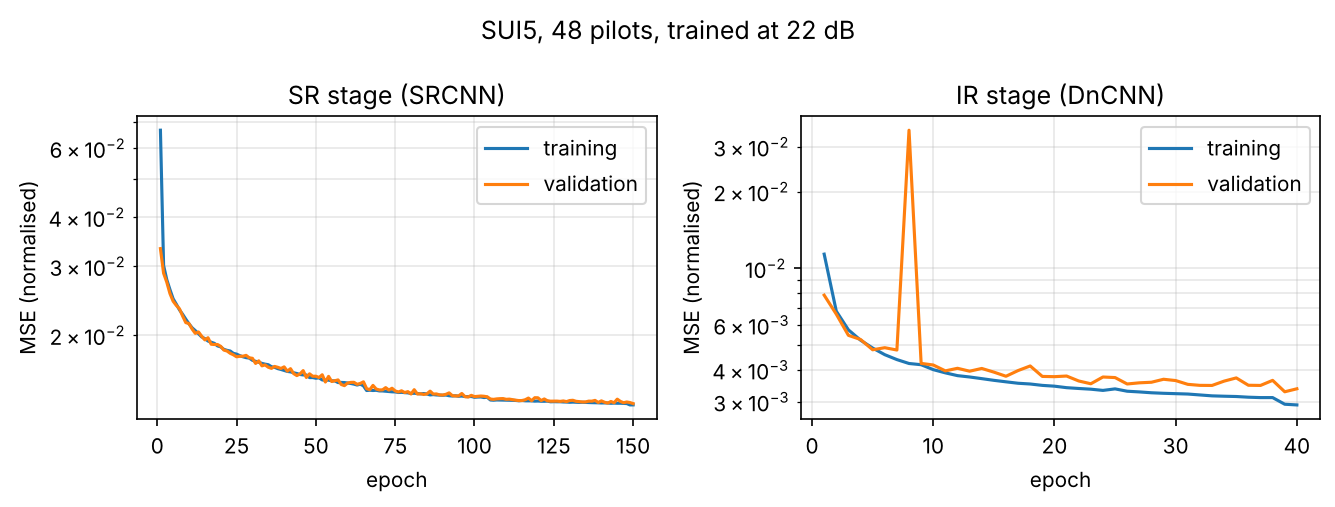
\includegraphics[width=\linewidth]{figures/loss_curves/loss_SUI5_p48_snr22.png}
    \caption{SUI5, 48 pilots, 22~dB.}
  \end{subfigure}
  \caption{Training and validation loss of the SR and IR stages. The curves of all 14 networks
    are in \code{results/figures/loss\_curves/}.}
  \label{fig:loss}
\end{figure}

% ---------------------------------------------------------------------------------------------
\section{Results (Task 6)}

All results use the 4\,000 test frames. Abbreviations in the tables: LS-lin = LS + linear
interpolation; SR-$s$ = SRCNN output alone; CN-$s$ = full ChannelNet trained at $s$~dB (``mix'' =
multi-SNR). \textbf{Bold} marks the best estimator that does not rely on genie statistics.

\subsection{MSE versus SNR (paper Figs.~3 and 4)}

\begin{figure}[!htbp]
  \centering
  \begin{subfigure}[t]{0.49\textwidth}
    \centering
    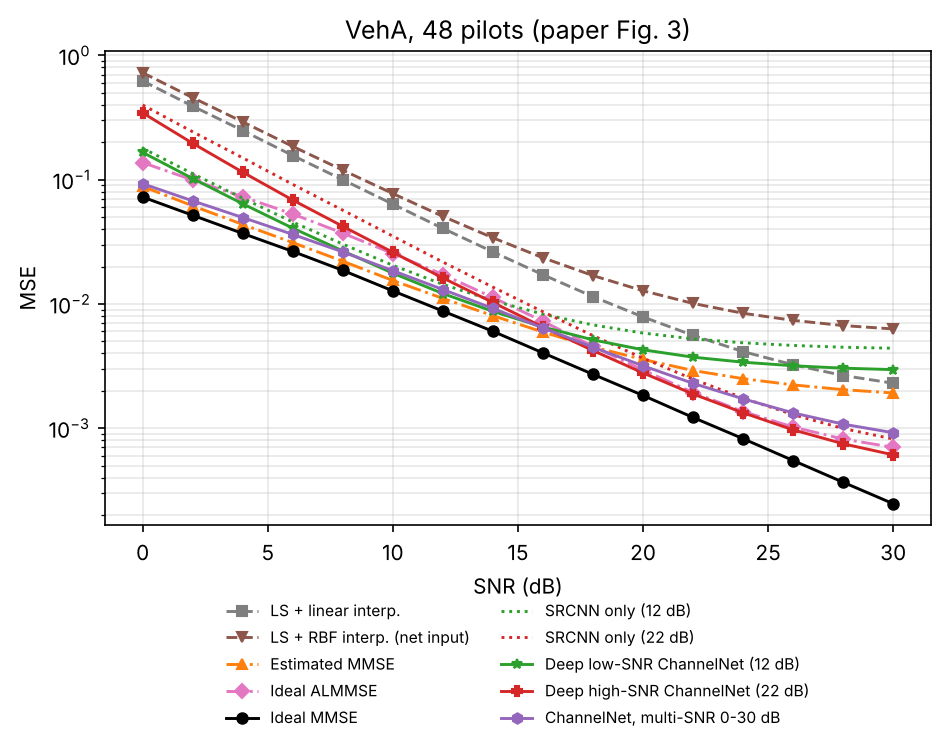
\includegraphics[width=\linewidth]{figures/fig3_VehA_mse_vs_snr.png}
    \caption{VehA (paper Fig.~3).}
  \end{subfigure}\hfill
  \begin{subfigure}[t]{0.49\textwidth}
    \centering
    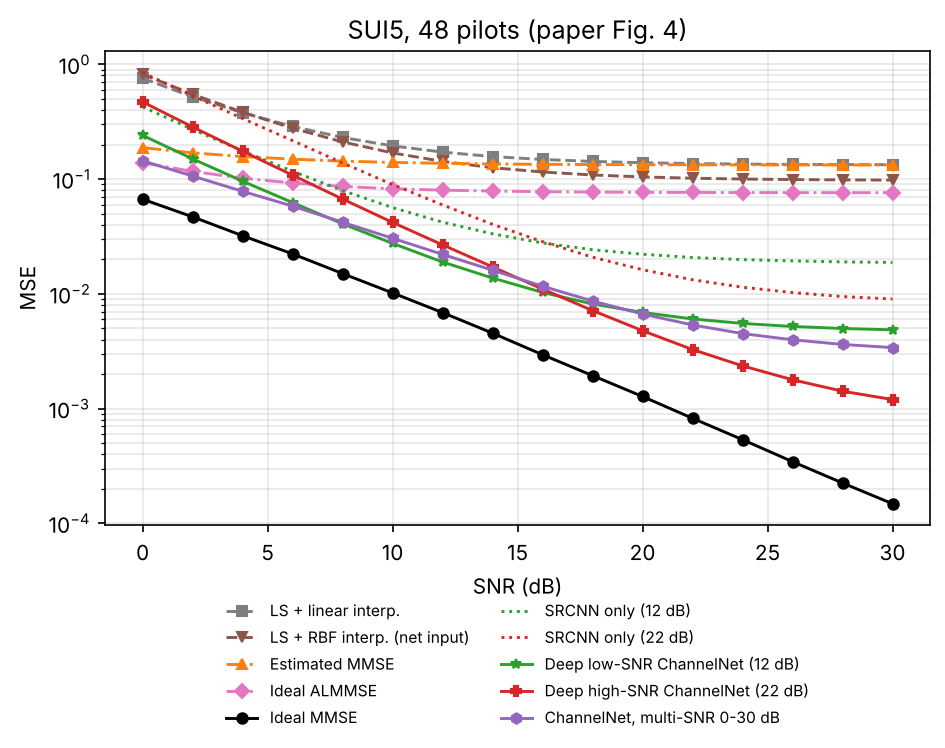
\includegraphics[width=\linewidth]{figures/fig4_SUI5_mse_vs_snr.png}
    \caption{SUI5 (paper Fig.~4).}
  \end{subfigure}
  \caption{MSE versus SNR with 48 pilots.}
  \label{fig:mse_snr}
\end{figure}

\begin{table}[!htbp]
  \centering
  \caption{MSE versus SNR, 48 pilots (selected SNRs).}
  \label{tab:snr}
  \footnotesize
  \setlength{\tabcolsep}{4pt}
\begin{tabular}{llcccccccc}
\toprule
channel & SNR (dB) & LS-lin & Est.\ MMSE & Ideal ALMMSE & Ideal MMSE & SR-22 & CN-12 & CN-22 & CN-mix \\
\midrule
VehA & 0 & $6.23\cdot10^{-1}$ & $\mathbf{8.82\cdot10^{-2}}$ & $1.37\cdot10^{-1}$ & $7.25\cdot10^{-2}$ & $3.99\cdot10^{-1}$ & $1.66\cdot10^{-1}$ & $3.45\cdot10^{-1}$ & $9.28\cdot10^{-2}$ \\
VehA & 6 & $1.56\cdot10^{-1}$ & $\mathbf{3.11\cdot10^{-2}}$ & $5.29\cdot10^{-2}$ & $2.65\cdot10^{-2}$ & $9.16\cdot10^{-2}$ & $4.07\cdot10^{-2}$ & $6.85\cdot10^{-2}$ & $3.62\cdot10^{-2}$ \\
VehA & 12 & $4.05\cdot10^{-2}$ & $\mathbf{1.11\cdot10^{-2}}$ & $1.72\cdot10^{-2}$ & $8.76\cdot10^{-3}$ & $2.17\cdot10^{-2}$ & $1.21\cdot10^{-2}$ & $1.62\cdot10^{-2}$ & $1.31\cdot10^{-2}$ \\
VehA & 20 & $7.85\cdot10^{-3}$ & $3.57\cdot10^{-3}$ & $2.94\cdot10^{-3}$ & $1.83\cdot10^{-3}$ & $3.66\cdot10^{-3}$ & $4.27\cdot10^{-3}$ & $\mathbf{2.78\cdot10^{-3}}$ & $3.18\cdot10^{-3}$ \\
VehA & 22 & $5.58\cdot10^{-3}$ & $2.91\cdot10^{-3}$ & $1.94\cdot10^{-3}$ & $1.22\cdot10^{-3}$ & $2.48\cdot10^{-3}$ & $3.73\cdot10^{-3}$ & $\mathbf{1.88\cdot10^{-3}}$ & $2.29\cdot10^{-3}$ \\
VehA & 30 & $2.30\cdot10^{-3}$ & $1.92\cdot10^{-3}$ & $7.01\cdot10^{-4}$ & $2.47\cdot10^{-4}$ & $8.18\cdot10^{-4}$ & $2.96\cdot10^{-3}$ & $\mathbf{6.10\cdot10^{-4}}$ & $9.19\cdot10^{-4}$ \\
\midrule
SUI5 & 0 & $7.55\cdot10^{-1}$ & $1.88\cdot10^{-1}$ & $1.39\cdot10^{-1}$ & $6.68\cdot10^{-2}$ & $8.46\cdot10^{-1}$ & $2.40\cdot10^{-1}$ & $4.70\cdot10^{-1}$ & $\mathbf{1.44\cdot10^{-1}}$ \\
SUI5 & 6 & $2.88\cdot10^{-1}$ & $1.49\cdot10^{-1}$ & $9.25\cdot10^{-2}$ & $2.23\cdot10^{-2}$ & $2.16\cdot10^{-1}$ & $6.24\cdot10^{-2}$ & $1.08\cdot10^{-1}$ & $\mathbf{5.82\cdot10^{-2}}$ \\
SUI5 & 12 & $1.72\cdot10^{-1}$ & $1.37\cdot10^{-1}$ & $8.01\cdot10^{-2}$ & $6.86\cdot10^{-3}$ & $5.96\cdot10^{-2}$ & $\mathbf{1.90\cdot10^{-2}}$ & $2.67\cdot10^{-2}$ & $2.21\cdot10^{-2}$ \\
SUI5 & 20 & $1.39\cdot10^{-1}$ & $1.33\cdot10^{-1}$ & $7.67\cdot10^{-2}$ & $1.27\cdot10^{-3}$ & $1.62\cdot10^{-2}$ & $6.89\cdot10^{-3}$ & $\mathbf{4.77\cdot10^{-3}}$ & $6.67\cdot10^{-3}$ \\
SUI5 & 22 & $1.37\cdot10^{-1}$ & $1.33\cdot10^{-1}$ & $7.65\cdot10^{-2}$ & $8.23\cdot10^{-4}$ & $1.33\cdot10^{-2}$ & $6.04\cdot10^{-3}$ & $\mathbf{3.27\cdot10^{-3}}$ & $5.36\cdot10^{-3}$ \\
SUI5 & 30 & $1.33\cdot10^{-1}$ & $1.33\cdot10^{-1}$ & $7.62\cdot10^{-2}$ & $1.48\cdot10^{-4}$ & $9.02\cdot10^{-3}$ & $4.86\cdot10^{-3}$ & $\mathbf{1.20\cdot10^{-3}}$ & $3.40\cdot10^{-3}$ \\
\bottomrule
\end{tabular}
\end{table}

\subsection{Deep high-SNR case: VehA and SUI5 separately}

\begin{figure}[!htbp]
  \centering
  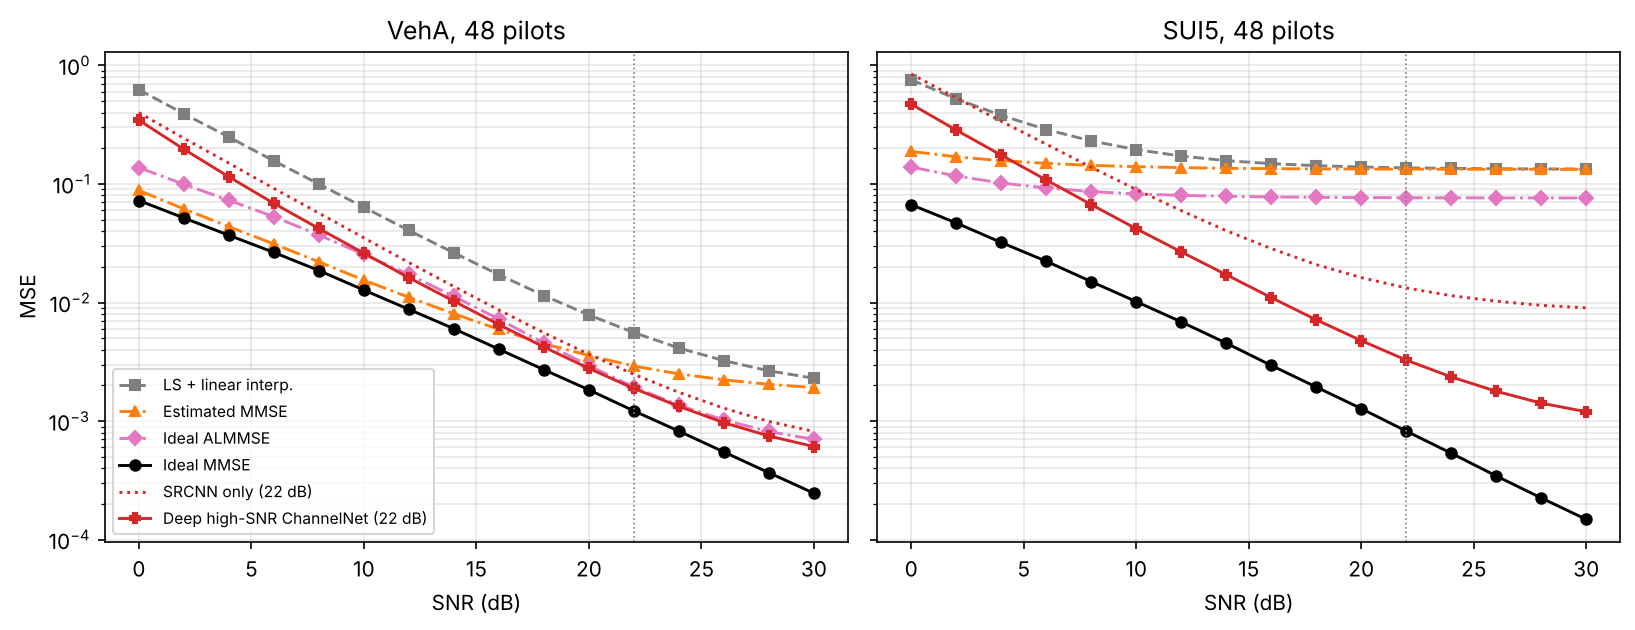
\includegraphics[width=0.86\textwidth]{figures/high_snr_VehA_vs_SUI5.png}
  \caption{Deep high-SNR ChannelNet (trained at 22~dB, marked by the vertical dotted line) against the
    baselines: VehA (left) and SUI5 (right).}
  \label{fig:highsnr}
\end{figure}

\subsection{MSE versus number of pilots (paper Fig.~5)}

\begin{figure}[!htbp]
  \centering
  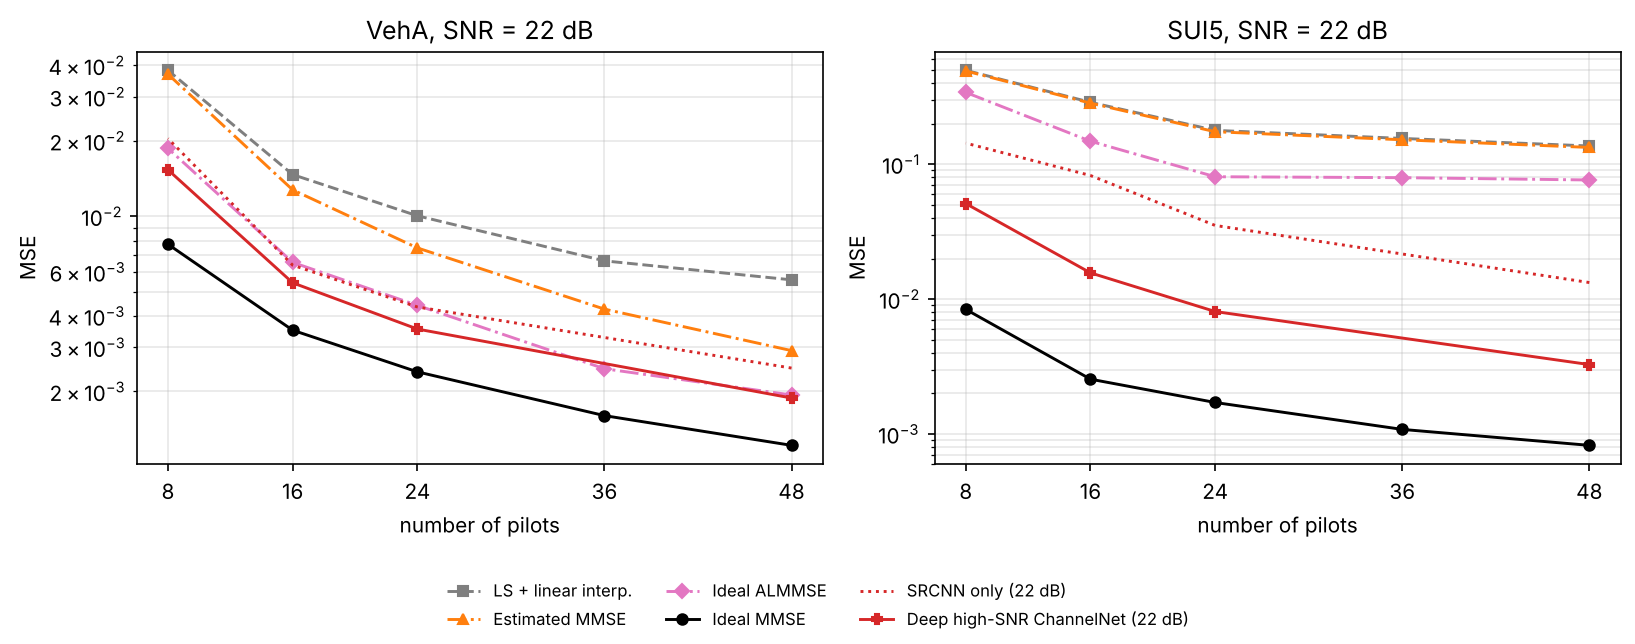
\includegraphics[width=0.86\textwidth]{figures/fig5_mse_vs_pilots_snr22.png}
  \caption{MSE versus number of pilots at 22~dB; a separate ChannelNet is trained at 22~dB for each
    density.}
  \label{fig:pilotsweep}
\end{figure}

\begin{table}[!htbp]
  \centering
  \caption{MSE versus number of pilots at 22~dB (36 pilots: baselines only).}
  \label{tab:pilots}
  \footnotesize
\begin{tabular}{llcccccc}
\toprule
channel & pilots & LS-lin & Est.\ MMSE & Ideal ALMMSE & Ideal MMSE & SR-22 & CN-22 \\
\midrule
VehA & 48 & $5.58\cdot10^{-3}$ & $2.91\cdot10^{-3}$ & $1.94\cdot10^{-3}$ & $1.22\cdot10^{-3}$ & $2.48\cdot10^{-3}$ & $\mathbf{1.88\cdot10^{-3}}$ \\
VehA & 36 & $6.64\cdot10^{-3}$ & $\mathbf{4.26\cdot10^{-3}}$ & $2.46\cdot10^{-3}$ & $1.60\cdot10^{-3}$ & -- & -- \\
VehA & 24 & $1.00\cdot10^{-2}$ & $7.48\cdot10^{-3}$ & $4.41\cdot10^{-3}$ & $2.40\cdot10^{-3}$ & $4.35\cdot10^{-3}$ & $\mathbf{3.55\cdot10^{-3}}$ \\
VehA & 16 & $1.47\cdot10^{-2}$ & $1.28\cdot10^{-2}$ & $6.55\cdot10^{-3}$ & $3.51\cdot10^{-3}$ & $6.39\cdot10^{-3}$ & $\mathbf{5.43\cdot10^{-3}}$ \\
VehA & 8 & $3.83\cdot10^{-2}$ & $3.69\cdot10^{-2}$ & $1.87\cdot10^{-2}$ & $7.74\cdot10^{-3}$ & $2.04\cdot10^{-2}$ & $\mathbf{1.53\cdot10^{-2}}$ \\
\midrule
SUI5 & 48 & $1.37\cdot10^{-1}$ & $1.33\cdot10^{-1}$ & $7.65\cdot10^{-2}$ & $8.23\cdot10^{-4}$ & $1.33\cdot10^{-2}$ & $\mathbf{3.27\cdot10^{-3}}$ \\
SUI5 & 36 & $1.55\cdot10^{-1}$ & $\mathbf{1.52\cdot10^{-1}}$ & $7.96\cdot10^{-2}$ & $1.08\cdot10^{-3}$ & -- & -- \\
SUI5 & 24 & $1.78\cdot10^{-1}$ & $1.74\cdot10^{-1}$ & $8.08\cdot10^{-2}$ & $1.71\cdot10^{-3}$ & $3.52\cdot10^{-2}$ & $\mathbf{8.09\cdot10^{-3}}$ \\
SUI5 & 16 & $2.88\cdot10^{-1}$ & $2.84\cdot10^{-1}$ & $1.48\cdot10^{-1}$ & $2.55\cdot10^{-3}$ & $8.26\cdot10^{-2}$ & $\mathbf{1.57\cdot10^{-2}}$ \\
SUI5 & 8 & $4.98\cdot10^{-1}$ & $4.92\cdot10^{-1}$ & $3.41\cdot10^{-1}$ & $8.40\cdot10^{-3}$ & $1.44\cdot10^{-1}$ & $\mathbf{5.11\cdot10^{-2}}$ \\
\bottomrule
\end{tabular}
\end{table}

\subsection{Cross-check on Vienna-simulator channels}
\label{sec:vienna}

The six 48-pilot ChannelNets were trained only on the Python channels. I tested them unchanged on 1\,000
frames from the Vienna 5G simulator, with the baselines using covariances from Vienna training frames
(\code{configs/vienna.yaml}). At every SNR their MSE is within \textbf{0.18~dB (VehA) and 0.32~dB
(SUI5)} of the matched-data result. For example, the deep high-SNR network at 22~dB reaches
$1.94\cdot10^{-3}$ instead of $1.88\cdot10^{-3}$ on VehA, and $3.39\cdot10^{-3}$ instead of
$3.27\cdot10^{-3}$ on SUI5. The ranking of all methods is unchanged. The networks depend on the channel
statistics rather than on the simulator that produced them, so the conclusions carry over to the
Vienna channels used in the paper.

\subsection{Inferences}

\begin{enumerate}
  \item \textbf{VehA} (Fig.~\ref{fig:mse_snr}a, paper Fig.~3). ChannelNet is about 5~dB better than LS
    + linear interpolation at every SNR. At their own training SNRs, the 12~dB and 22~dB networks are
    within 1.4~dB and 1.9~dB of the genie ideal MMSE. They beat the ideal ALMMSE from 4~dB upwards and
    the estimated MMSE from 18~dB upwards (by 1.9~dB at 22~dB). Below 12~dB my estimated MMSE, whose
    covariance comes from 2\,000 frames, is 0.3--2.7~dB better than ChannelNet, so the paper's
    ``comparable with the ideal MMSE'' at low SNR is reproduced only approximately. At medium and high
    SNR the ordering ideal MMSE $<$ ChannelNet $<$ ALMMSE/estimated MMSE $<$ LS is the same as in the
    paper.
  \item \textbf{SUI5} (Fig.~\ref{fig:mse_snr}b, paper Fig.~4). With a 10~$\mu$s delay spread, the
    frequency response changes faster than a pilot every 6 sub-carriers can follow. Every estimator
    that starts from an interpolated grid therefore hits an error floor from about 10~dB: 0.13 for LS
    and the estimated MMSE, 0.077 for the ideal ALMMSE. The paper shows the same behaviour.
    ChannelNet keeps improving, reaching $3.3\cdot10^{-3}$ at 22~dB and $1.2\cdot10^{-3}$ at 30~dB.
    At 22~dB it is 16~dB better than the estimated MMSE and 13.7~dB better than the ideal ALMMSE
    (Fig.~\ref{fig:highsnr}). Only the ideal MMSE, which applies the exact 2-D covariance directly to
    the pilots, does better.
  \item \textbf{SNR-specific networks.} The 22~dB network overtakes the 12~dB one above 16~dB (VehA) and
    18~dB (SUI5); this is where the paper switches between its two networks. Away from its training
    SNR each network degrades. The 12~dB VehA model levels off near $3\cdot10^{-3}$ and is worse than
    plain LS at 28--30~dB. The 22~dB model is 6.8~dB above the ideal MMSE at 0~dB.
  \item \textbf{Contribution of the DnCNN.} The SRCNN output is already 5--9~dB better than its
    RBF-interpolated input. The DnCNN adds a further 0.3--1.7~dB on VehA but 2.5--8.8~dB on SUI5,
    where the SRCNN alone saturates at $9\cdot10^{-3}$ (30~dB). The two-stage design of the paper
    matters most for the harder channel.
  \item \textbf{Pilot density} (Fig.~\ref{fig:pilotsweep}, paper Fig.~5). As in the paper, ChannelNet
    beats the estimated MMSE and the ideal ALMMSE at every density. On VehA it reaches
    $1.9/3.5/5.4/15\cdot10^{-3}$ for 48/24/16/8 pilots, against $2.9/7.5/13/37\cdot10^{-3}$ for the
    estimated MMSE. Its gap to the ideal MMSE grows from 1.9 to 3.0~dB as pilots are removed. On SUI5,
    ChannelNet with only 16 pilots is still 9~dB better than the estimated MMSE with 48, i.e.\ it needs
    about a third of the pilot overhead.
  \item \textbf{Multi-SNR training.} A single network trained over 0--30~dB stays within about 1~dB of
    the better SNR-specific network from 8 to 22~dB, and beats both below 8~dB by up to 2.5~dB. It
    loses up to 1.8~dB (VehA) and 4.5~dB (SUI5) at high SNR (Section~\ref{sec:discussion}).
\end{enumerate}

% ---------------------------------------------------------------------------------------------
\section{Discussion: SNR-specific training and generalisation}
\label{sec:discussion}

\begin{figure}[!htbp]
  \centering
  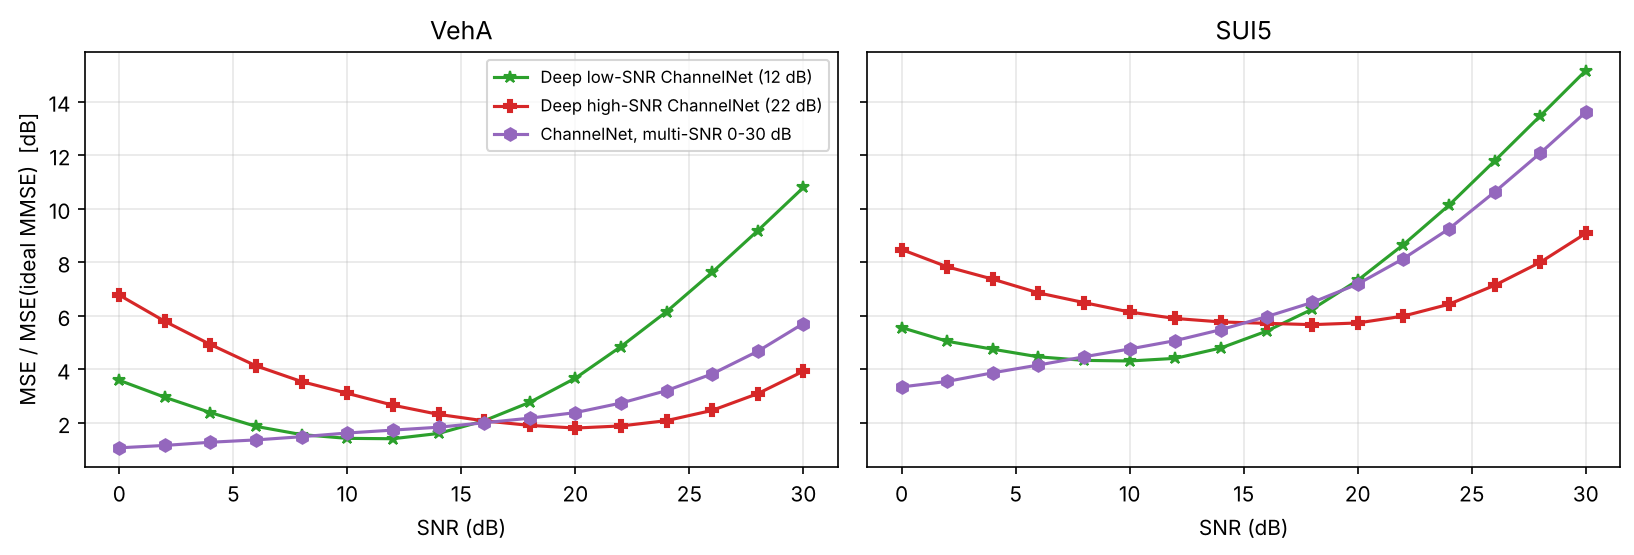
\includegraphics[width=0.86\textwidth]{figures/snr_generalization.png}
  \caption{Excess MSE of each ChannelNet over the ideal MMSE (dB) across SNR, 48 pilots. Each
    SNR-specific network is best only near its training SNR.}
  \label{fig:gen}
\end{figure}

\paragraph{Limitations of training at one SNR.} The paper itself notes that the best weights depend
on the SNR, and that training a network for every SNR is impractical because the SNR is continuous.
It therefore uses two networks and observes that the high-SNR network starts to fail again above about
23~dB. My results show the same effects (Fig.~\ref{fig:gen}):
\begin{enumerate}
  \item \emph{Noise-level mismatch (covariate shift).} The DnCNN learns to remove noise of one
    particular strength. Below its training SNR the input is noisier than anything it saw, and it
    removes too little: the 22~dB VehA model is 6.8~dB above the ideal MMSE at 0~dB.
  \item \emph{Over-smoothing and error floors.} Above its training SNR the network keeps removing
    ``noise'' that is in fact channel detail. The 12~dB VehA model flattens at about $3\cdot10^{-3}$
    and is worse than plain LS at 28--30~dB. The gap of the 22~dB model to the ideal MMSE grows from
    1.9~dB at 22~dB to 3.9~dB at 30~dB. The SR stage behaves the same way, because it learns an
    SNR-dependent, Wiener-like amount of smoothing.
  \item \emph{Practical cost.} A deployment needs several networks, an SNR estimator and a switching
    rule, and an SNR estimation error selects the wrong network. The same over-specialisation applies
    to the pilot pattern, Doppler and delay spread: each of my 14 networks is valid for one (channel,
    pattern, SNR) combination only.
\end{enumerate}

\paragraph{Ways to generalise across SNR.}
\begin{enumerate}
  \item \textbf{Blind multi-SNR training}, as in DnCNN-B~\cite{dncnn} and ReEsNet~\cite{reesnet}
    (\emph{implemented here}). One network sees all noise levels during training. It is within about
    1~dB of the better SNR-specific model from 8 to 22~dB and the best of the three below 8~dB. It
    loses up to 1.8/4.5~dB (VehA/SUI5) at high SNR because its capacity is shared across noise levels.
  \item \textbf{Noise-level conditioning.} The estimated noise level is given to the network, either as
    an extra input map (FFDNet~\cite{ffdnet}) or through feature-wise modulation (FiLM~\cite{film}).
    One network can then adjust its denoising strength continuously.
  \item \textbf{SNR bank / mixture of experts.} A few networks, each trained on one SNR bin, are
    selected with an SNR estimate. This is the strategy of the paper; my results put the switch at
    the 16--18~dB crossover.
  \item \textbf{Model-driven (unfolded) networks}, such as the learned denoising-based AMP of He
    \emph{et al.}~\cite{ldamp}, where the noise variance enters the algorithm explicitly as a parameter.
  \item \textbf{Curriculum learning and augmentation}~\cite{curriculum} over SNR, Doppler and delay
    spread; \textbf{untrained priors} such as the deep image prior~\cite{dip}, which need no training
    SNR at all; and \textbf{learned pilot patterns}~\cite{pilotdesign}, which reduce the sensitivity to
    pilot density.
\end{enumerate}

\paragraph{Other limitations.} Inter-carrier interference (Doppler) and inter-symbol interference
(SUI5 delay $>$ CP) are not modelled: the ground truth is the channel at each symbol centre and
$Y=HX+Z$. The ideal MMSE and ALMMSE use genie statistics. The pilot study was run at 22~dB, the deep
high-SNR operating point, instead of the paper's 20~dB. The DnCNN (0.67\,M parameters, about 2.7~GFLOP
per frame) is far more expensive than a $1008\times48$ LMMSE matrix product.

% ---------------------------------------------------------------------------------------------
\section{Conclusion}

Treating the $72\times14$ channel grid as an image, ChannelNet reconstructs it from 48 noisy pilots by
super-resolution followed by denoising. On VehA it is about 5~dB better than LS interpolation at every
SNR, within 1.4--1.9~dB of the genie ideal MMSE at its training SNRs, and better than the estimated
MMSE above 18~dB. On the long-delay SUI5 channel, every practical linear estimator saturates at
0.08--0.13, while ChannelNet keeps improving down to $1.2\cdot10^{-3}$ (16~dB better than the
estimated MMSE at 22~dB), in line with the paper. Its main weakness is its dependence on the training
SNR, which shows up as error floors and a crossover at 16--18~dB. Multi-SNR training removes most of
this with a single network, and noise-level conditioning is the natural next step.

% ---------------------------------------------------------------------------------------------
{\small
\begin{thebibliography}{99}\setlength{\itemsep}{0pt}
\bibitem{soltani} M.~Soltani, V.~Pourahmadi, A.~Mirzaei, H.~Sheikhzadeh, ``Deep learning-based channel
  estimation,'' \emph{IEEE Commun. Lett.}, vol.~23, no.~4, pp.~652--655, 2019 (arXiv:1810.05893v4).
\bibitem{srcnn} C.~Dong, C.~C.~Loy, K.~He, X.~Tang, ``Image super-resolution using deep convolutional
  networks,'' \emph{IEEE TPAMI}, vol.~38, no.~2, 2016.
\bibitem{dncnn} K.~Zhang, W.~Zuo, Y.~Chen, D.~Meng, L.~Zhang, ``Beyond a Gaussian denoiser: residual
  learning of deep CNN for image denoising,'' \emph{IEEE TIP}, vol.~26, no.~7, 2017.
\bibitem{simko} M.~\v{S}imko, C.~Mehlf\"uhrer, M.~Wrulich, M.~Rupp, ``Doubly dispersive channel
  estimation with scalable complexity,'' \emph{Proc. WSA}, 2010.
\bibitem{zheng} Y.~R.~Zheng, C.~Xiao, ``Simulation models with correct statistical properties for
  Rayleigh fading channels,'' \emph{IEEE Trans. Commun.}, vol.~51, no.~6, 2003.
\bibitem{reesnet} L.~Li, H.~Chen, H.-H.~Chang, L.~Liu, ``Deep residual learning meets OFDM channel
  estimation,'' \emph{IEEE Wireless Commun. Lett.}, vol.~9, no.~5, 2020.
\bibitem{ffdnet} K.~Zhang, W.~Zuo, L.~Zhang, ``FFDNet: toward a fast and flexible solution for CNN-based
  image denoising,'' \emph{IEEE TIP}, vol.~27, no.~9, 2018.
\bibitem{film} E.~Perez, F.~Strub, H.~de~Vries, V.~Dumoulin, A.~Courville, ``FiLM: visual reasoning with a
  general conditioning layer,'' \emph{Proc. AAAI}, 2018.
\bibitem{ldamp} H.~He, C.-K.~Wen, S.~Jin, G.~Y.~Li, ``Deep learning-based channel estimation for
  beamspace mmWave massive MIMO systems,'' \emph{IEEE Wireless Commun. Lett.}, vol.~7, no.~5, 2018.
\bibitem{curriculum} Y.~Bengio, J.~Louradour, R.~Collobert, J.~Weston, ``Curriculum learning,''
  \emph{Proc. ICML}, 2009.
\bibitem{dip} D.~Ulyanov, A.~Vedaldi, V.~Lempitsky, ``Deep image prior,'' \emph{Proc. CVPR}, 2018.
\bibitem{pilotdesign} M.~Soltani, V.~Pourahmadi, H.~Sheikhzadeh, ``Pilot pattern design for deep
  learning-based channel estimation in OFDM systems,'' \emph{IEEE Wireless Commun. Lett.}, vol.~9,
  no.~12, 2020.
\end{thebibliography}
}

\end{document}
